%! Author = Kiddo_Tsukuyomi
%! Date = 

% Preamble
\documentclass[UTF8]{ctexart}

% Packages
\usepackage{geometry}
\usepackage{listings}
\usepackage{xcolor}
\usepackage{graphicx}
\usepackage{amsmath}
\usepackage{subcaption}

% Settings
\lstset{
    backgroundcolor=\color{gray!5}, % Code block background color
    basicstyle=\ttfamily\small, % Font style: monospaced, small size
    columns=fullflexible, % Allow line wrapping, no restrictions on column number
    keepspaces=true, % Preserve spaces
    language=[LaTeX]TeX, % Code language is LaTeX
    breaklines=true, % Allow automatic line breaking
    breakatwhitespace=true, % Break at whitespace only
    postbreak=\mbox{\textcolor{red}{$\hookrightarrow$}\space}, % Mark break position with red arrow
    commentstyle=\color{gray}\itshape, % Comment style: gray italic
    stringstyle=\color{orange}, % String style: orange
    keywordstyle=\color{blue}, % Keyword style: blue
    showstringspaces=false, % Do not show spaces within strings
    numbers=left, % Display line numbers on the left
    numberstyle=\scriptsize, % Line number font size: footnote size
    numbersep=8pt, % Distance between line numbers and code: 8pt
    frame=single, % Add single line border
    frameround=tttt, % Rounded corners for the frame
    rulecolor=\color{black}, % Frame color: black
    extendedchars=true, % Allow the use of extended character sets
    inputencoding=utf8, % Input encoding: UTF-8
    literate={~} {$\sim$}{1}, % Handle tilde symbol display
    escapeinside=``, % Use backticks as an escape region, to avoid garbled characters when using Chinese text
    xleftmargin=2em, % Left margin of the code block
    xrightmargin=2em, % Right margin of the code block
    aboveskip=1em, % Space above the code block
    framexleftmargin=2em, % Left margin of the frame
}

% Document
\begin{document}
	\title{\textbf{HW15}}
	\author{白博臣、何骐多、夏营}
	\date{}
	\maketitle

    \begin{figure}[h]
        \centering
        \begin{minipage}{0.32\textwidth}
            \centering
            
\includegraphics[width=\linewidth]{bbc}
            \caption{白博臣}
            \label{fig:img1}
        \end{minipage}\hfill
        \begin{minipage}{0.305\textwidth}
            \centering
            \includegraphics[width=\linewidth]{hqd}
            \caption{何骐多}
            \label{fig:img2}
        \end{minipage}\hfill
        \begin{minipage}{0.32\textwidth}
            \centering
            
\includegraphics[width=\linewidth]{xy}
            \caption{夏营}
            \label{fig:img3}
        \end{minipage}
    \end{figure}

    \section{Problem1}\label{sec:1}
    当模拟一维 Ising 模型时,我们需要实现以下步骤:

    初始化系统:设置自旋格子数,外界温度T,外加磁场h,以及初始自旋构型

    计算能量:根据 Ising 模型的能量函数计算每种构型的能量。

    选择随机自旋:随机选择一个自旋进行翻转。

    计算翻转后的能量变化:计算翻转后系统能量与翻转之前能量的差值 ΔE。

    判断是否接受翻转:如果 \(\DeltaE < 0\),则接受翻转;否则,以概率 \(e^{-\DeltaE/kT}\) 接受翻转。

    重复上述步骤,直到系统达到平衡

    \subsection{a}\label{subsec:1.1}
    对于此题,我们初始设置自旋格子数为\(20\),外界温度为\(1.0 \frac{J}{k_B}\) ,外加磁场\(h=0\),以及初始所有自旋格子的自旋方向均为向上,即\(spin=1\)。

    由以下代码实现计算周期性边界的系统能量:
    \begin{lstlisting}[language=Python, breaklines = true,label={lst:1.1.1}]
def energy(spins, h):
    n = len(spins)
    energy = 0
    for i in range(n):
        energy += -(spins[(i - 1) % n] + spins[(i + 1) % n])*spin[i] - h * spins[i]
    return energy/2
    \end{lstlisting}

    以下代码实现随机选取一个格子进行翻转并利用Metropolis-Hastings算法来判断是否接受这一翻转结果:
    \begin{lstlisting}[language=Python, breaklines = true,label={lst:1.1.2}]
# `实现自旋翻转`
def flip(spins, beta):
    n = len(spins)
    # `随机选取翻转的自旋格子`
    i = np.random.randint(n)
    s = -spins[i]

    deltaE = 2 * spins[i] * (spins[(i - 1) % n] + spins[(i + 1) % n])
    if deltaE <= 0:
        spins[i] = s
    elif np.random.random() < np.exp(-beta * deltaE):
        spins[i] = s

    return spins
    \end{lstlisting}

    以下代码对MCMC算法模拟Ising model进行实际运算:
    \begin{lstlisting}[language=Python, breaklines = true,label={lst:1.1.3}]
# `实现MCMC算法`
def MCMC(spins, T, n, h):
    beta = 1.0 / T
    energies = np.array([])
    m = np.array([])
    for i in range(n):
        spins = flip(spins, beta)
        e = energy(spins, h)
        m = np.append(m, sum(spins))
        energies = np.append(energies, e)
    return energies, m
    \end{lstlisting}

    而后只需将初始设定的条件代入运算即可,结果如下:

    \begin{figure}[h]
        \centering
        \includegraphics[height=0.32 \textheight]{1.1.1}
        \label{fig:1.1.1}
    \end{figure}
    \begin{figure}[h]
        \centering
        \includegraphics[height=0.32 \textheight]{1.1.2}
        \label{fig:1.1.2}
    \end{figure}

    从图上我们可以大致的看出,在经历了\(100\)步左右,系统趋近于平衡状态。

    \subsection{b}\label{subsec:1.2}
    将自旋的初始构型随机给定,即每个自旋格子的自旋方向等可能的向上或者向下。我们利用\texttt{python numpy}库中的\texttt{random.choice([-1,1],size=N)}函数来实现这一条件,其余步骤与上一问相同,有结果如下:

    \begin{figure}[h]
        \centering
        \includegraphics[height=0.32 \textheight]{1.2.1}
        \label{fig:1.2.1}
    \end{figure}
    \begin{figure}[h]
        \centering
        \includegraphics[height=0.32 \textheight]{1.2.2}
        \label{fig:1.2.2}
    \end{figure}

    \subsection{c}\label{subsec:1.3}
    由以下代码实现对于T属于[0.5,5]区间的遍历,同时记录<E>,<M>的结果:
    \begin{lstlisting}[language=Python, breaklines = true,label={lst:1.3}]
for i in range(len(T)):
    e, m = MCMC(spin, T[i], 1000, 0)
    E = np.append(E, np.sum(e) / len(e))
    M = np.append(M, np.sum(m) / len(m))
    \end{lstlisting}

    基于此,可以绘出模拟中<E>,<M>与T的关系,同时有Ising model给出的<E>计算公式:
    \begin{equation*}
        <E> =-N\tanh{\frac{J}{k_B T}}
    \end{equation*}

    我们可以绘出理论曲线。

    具体结果实现如下:
    \begin{figure}[h]
        \centering
        \includegraphics[height=0.32 \textheight]{1.3.1}
        \label{fig:1.3.1}
    \end{figure}
    \begin{figure}[h]
        \centering
        \includegraphics[height=0.32 \textheight]{1.3.2}
        \label{fig:1.3.2}
    \end{figure}

    \subsection{d}\label{subsec:1.4}
    对于此题,我们只需要在实现自旋翻转的函数中增加一个值来记录其是否成功接受翻转即可,代码大致如下:
    \begin{lstlisting}[language=Python, breaklines = true,label={lst:1.4}]
# `实现自旋翻转`
def flip(spins, beta):
    n = len(spins)
    # `随机选取翻转的自旋格子`
    i = np.random.randint(n)
    s = -spins[i]
    accept = 0

    deltaE = 2 * spins[i] * (spins[(i - 1) % n] + spins[(i + 1) % n])
    if deltaE <= 0:
        spins[i] = s
        accept = 1
    elif np.random.random() < np.exp(-beta * deltaE):
        spins[i] = s
        accept = 1
    return spins, accept
    \end{lstlisting}

    我们增加了一个accept变量,当其为1时表示成功接受了这一翻转,为0则不接受。

    由此可以实现对MCMC算法中接受次数的统计,绘出结果图如下:

    \begin{figure}[h]
        \centering
        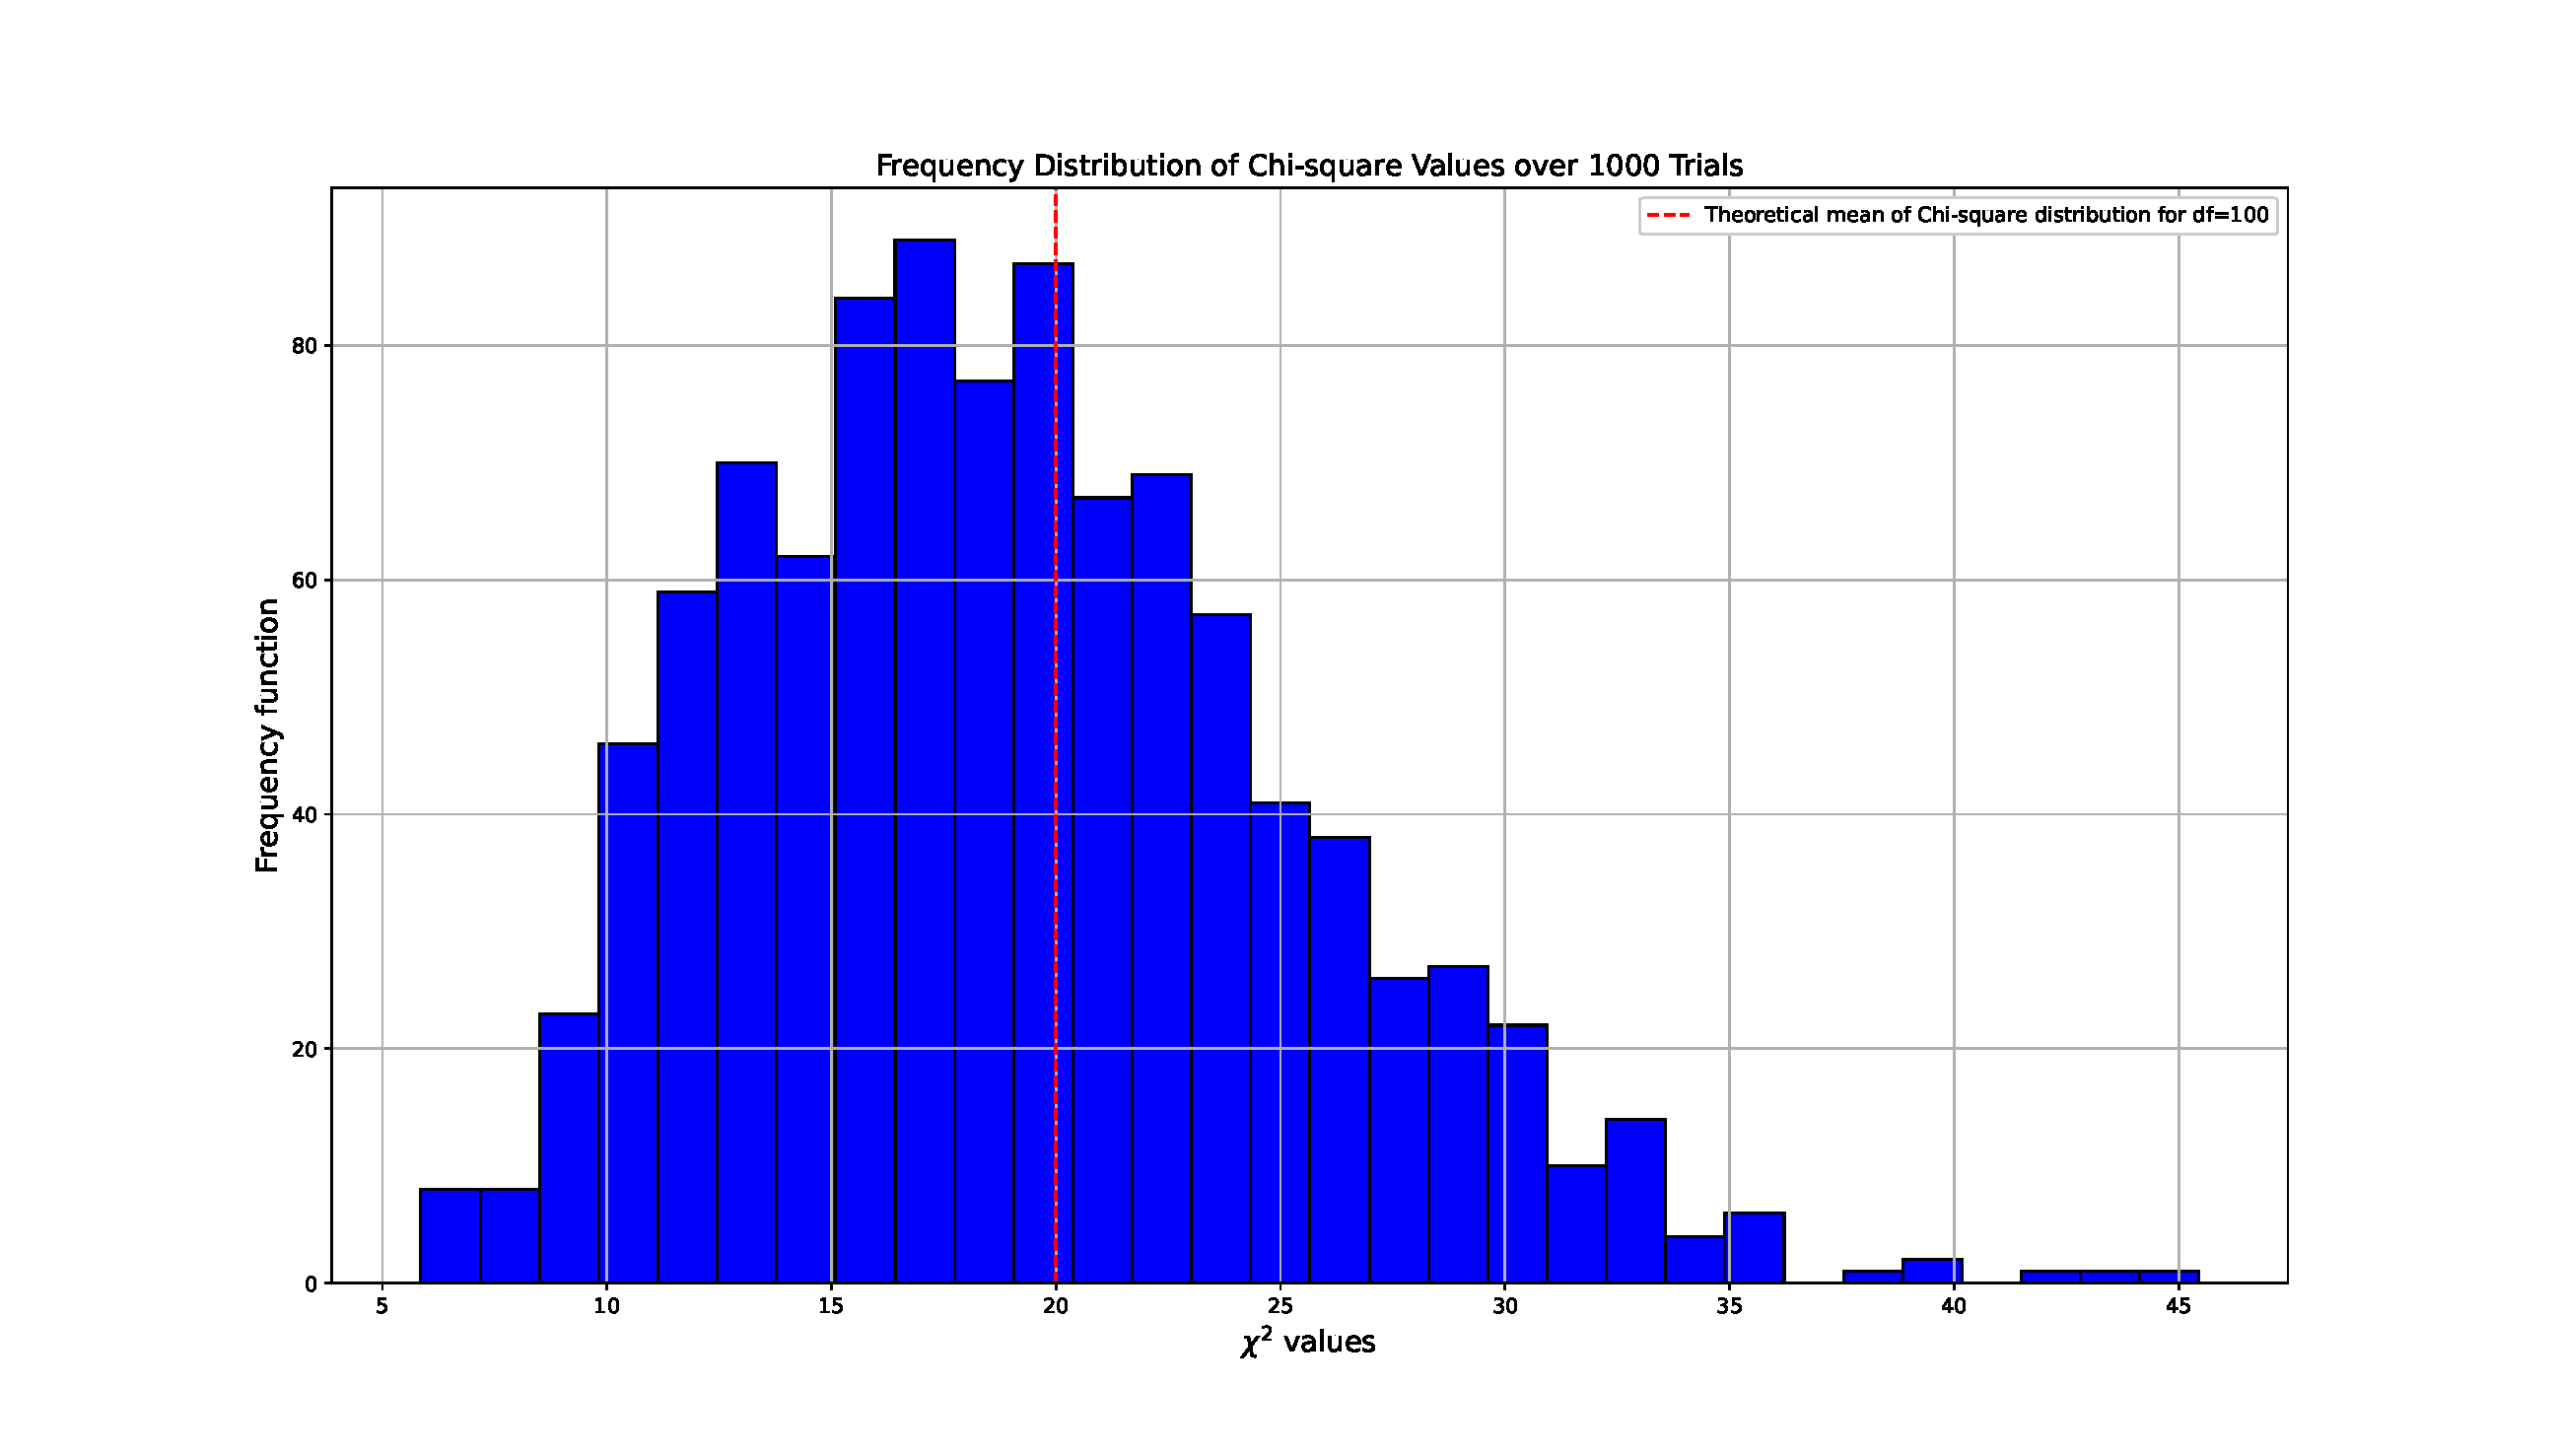
\includegraphics[height=0.32 \textheight]{1.4}
        \label{fig:1.4}
    \end{figure}

    可以发现,随着温度的升高,接受率也在逐渐的增高。

    在Metropolis算法中,T的接受率(acceptance rate)和增减幅度(rate of change)通常不是函数。它们取决于以下因素:

    温度(T):接受率和增减幅度会随温度的变化而变化。在高温下,接受率更高,系统更容易接受状态变化;而在低温下,接受率较低,系统更倾向于保持当前状态。

    能量差(ΔE):接受率也取决于状态变化引起的能量差。如果能量差较小(负数或接近零),则接受率更高;如果能量差较大(正数),则接受率较低。

    对于大都会算法(Metropolis-Hastings算法),在低温下的效率通常会降低。这是因为在低温下,系统更倾向于保持当前状态,而接受率较低。因此,在低温下,系统需要更多的步骤才能达到平衡状态,从而导致算法效率较低。在高温下,接受率较高,状态变化更频繁,系统更容易达到平衡状态,因此算法效率更高。

    \subsection{e}\label{subsec:1.5}
    对于此题,可以仿照上述对T的遍历实现对h值的遍历,对模拟模型函数进行了修改,以计算和存储平均磁化强度作为外部磁场(h)的函数。然后,我们对多个温度进行模拟,并将结果存储在磁化阵列中。最后,我们绘制了每个温度的磁化强度作为h的函数。实现结果如下:
    \begin{figure}[h]
        \centering
        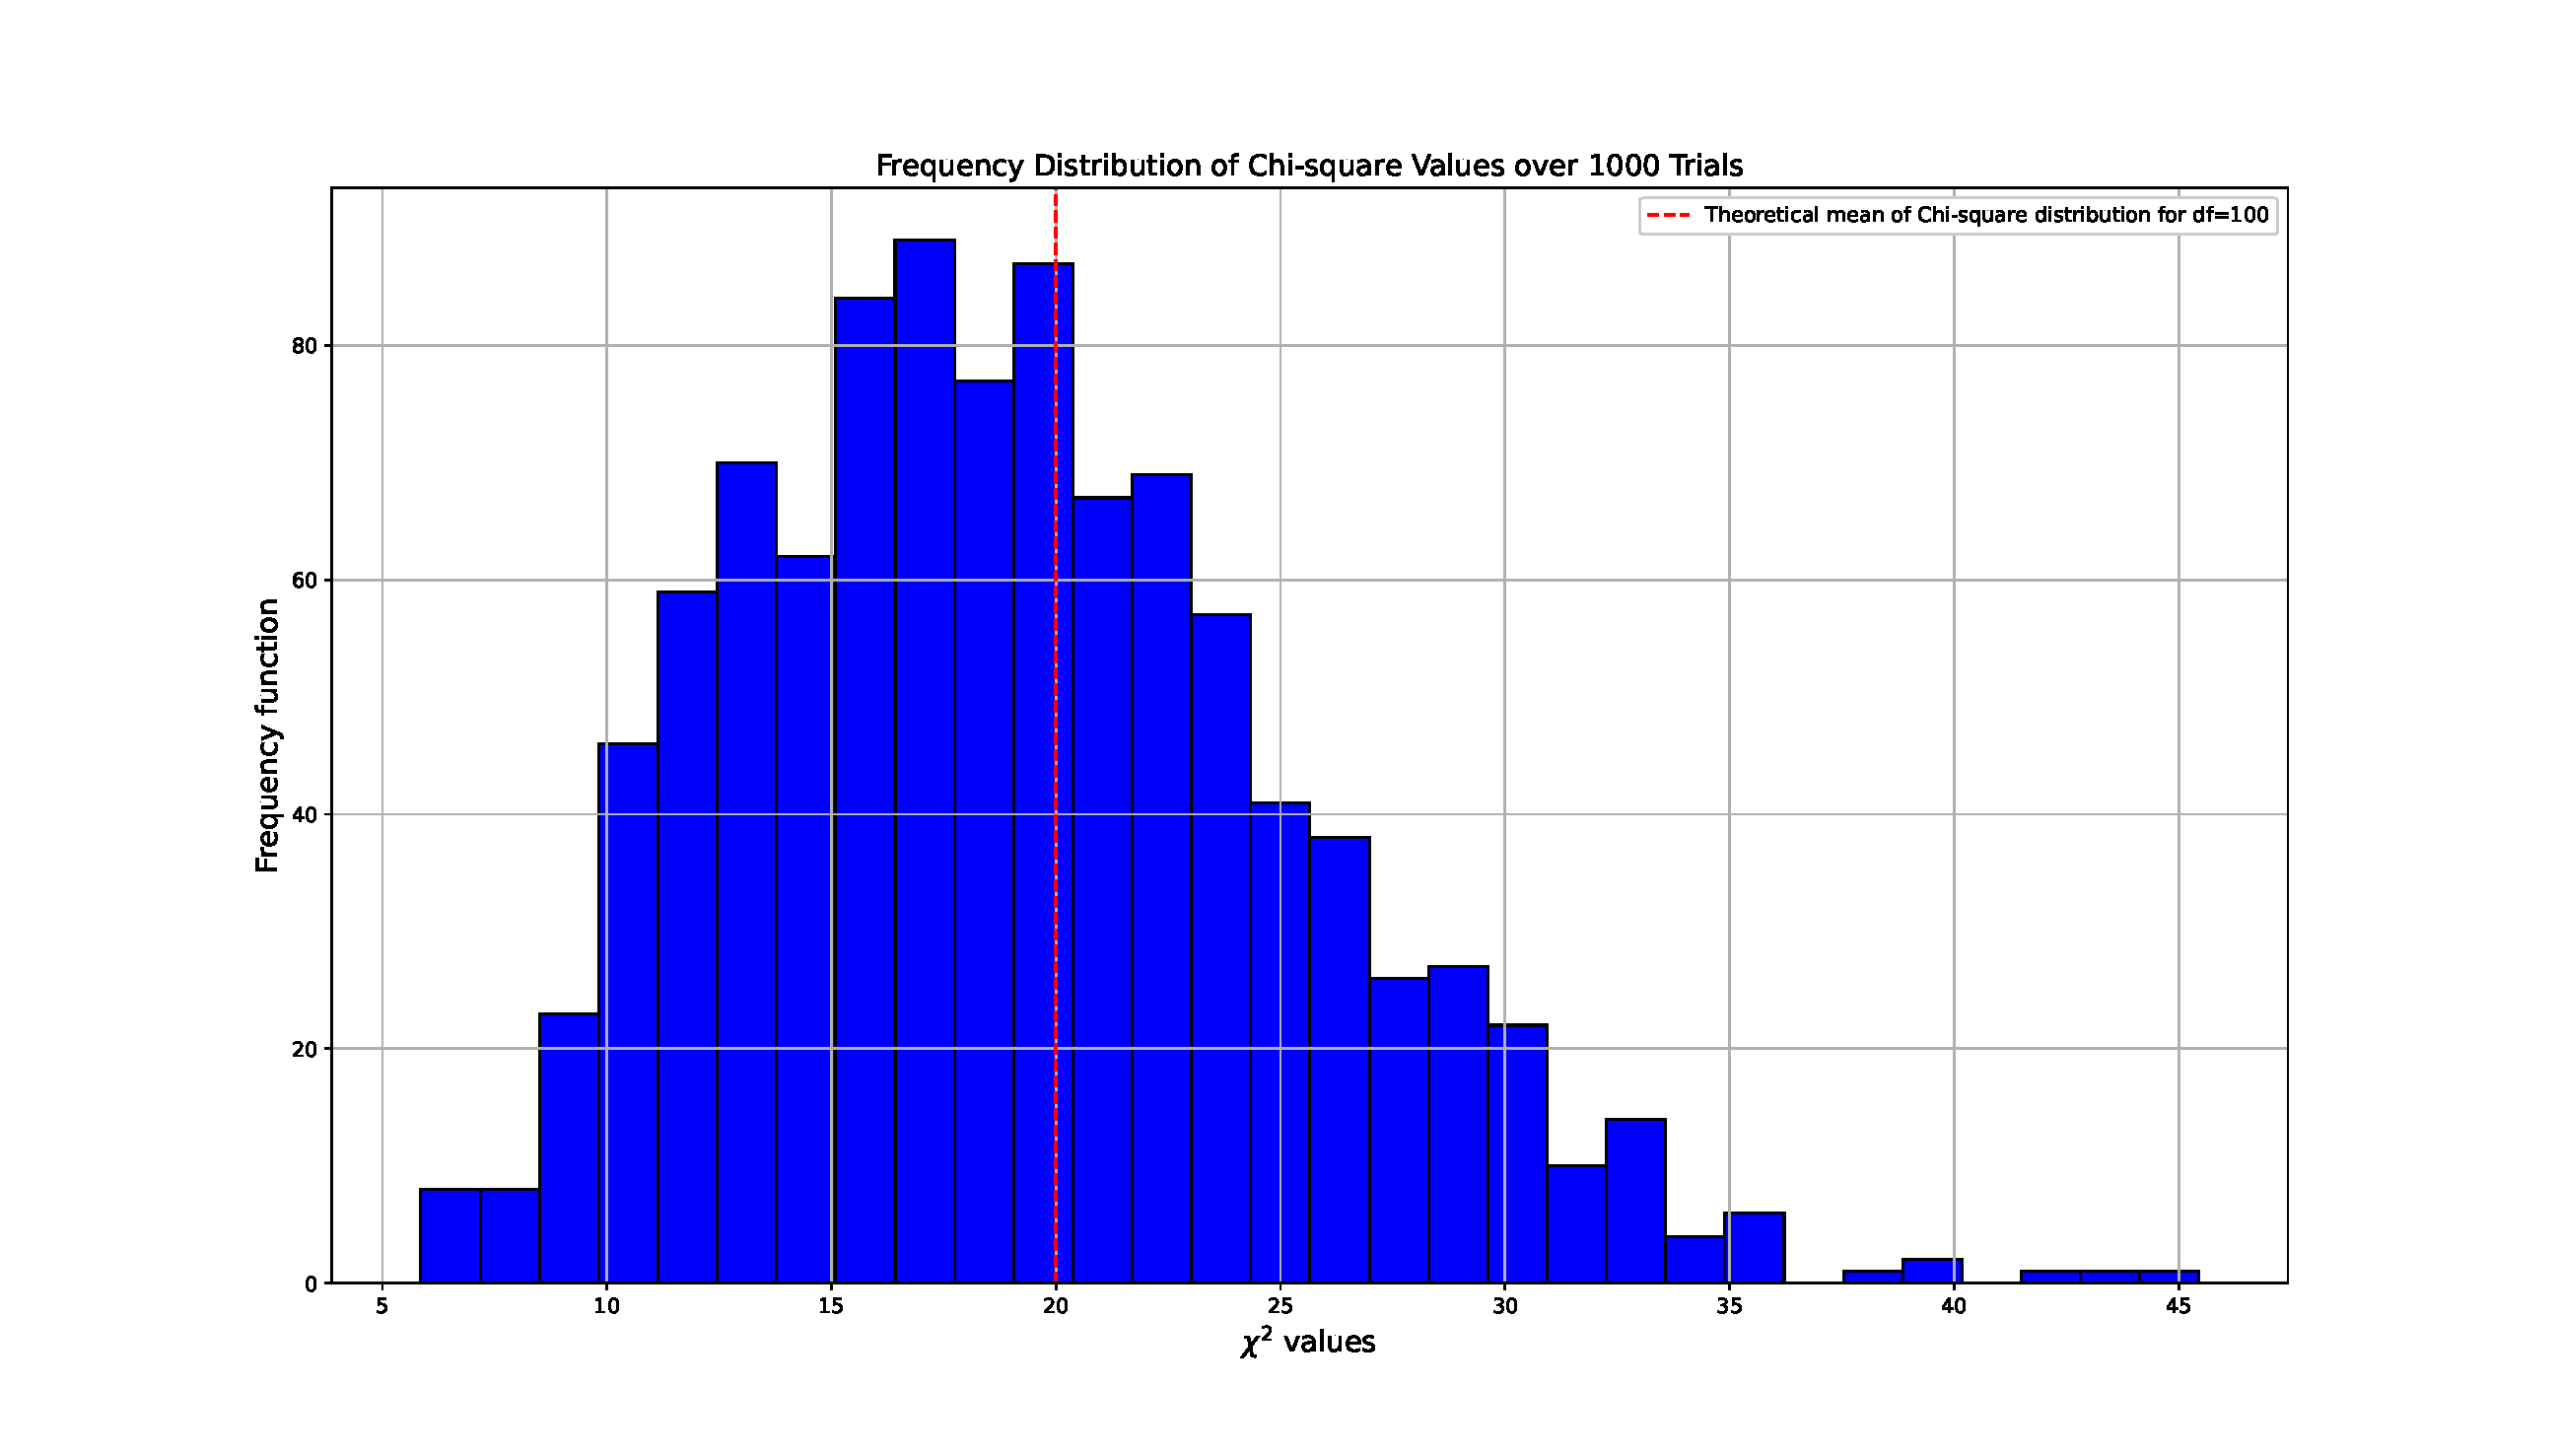
\includegraphics[height=0.32 \textheight]{1.5}
        \label{fig:1.5}
    \end{figure}

    通过对曲线图的分析,我们可以观察到不同温度下随外加磁场变化时的磁化行为。同时亦如问题所述,所有温度下h=0时的磁化强度应为零。

    \subsection{f}\label{subsec:1.6}
    与上一题类似,这里我们修改了模拟模型函数,但与之不同的是,我们这里固定T=1,并多个自旋格子数N进行了模拟,并将结果与理论结果,即N→∞时的结果进行了比较。

    具体结果如下:
    \begin{figure}[h]
        \centering
        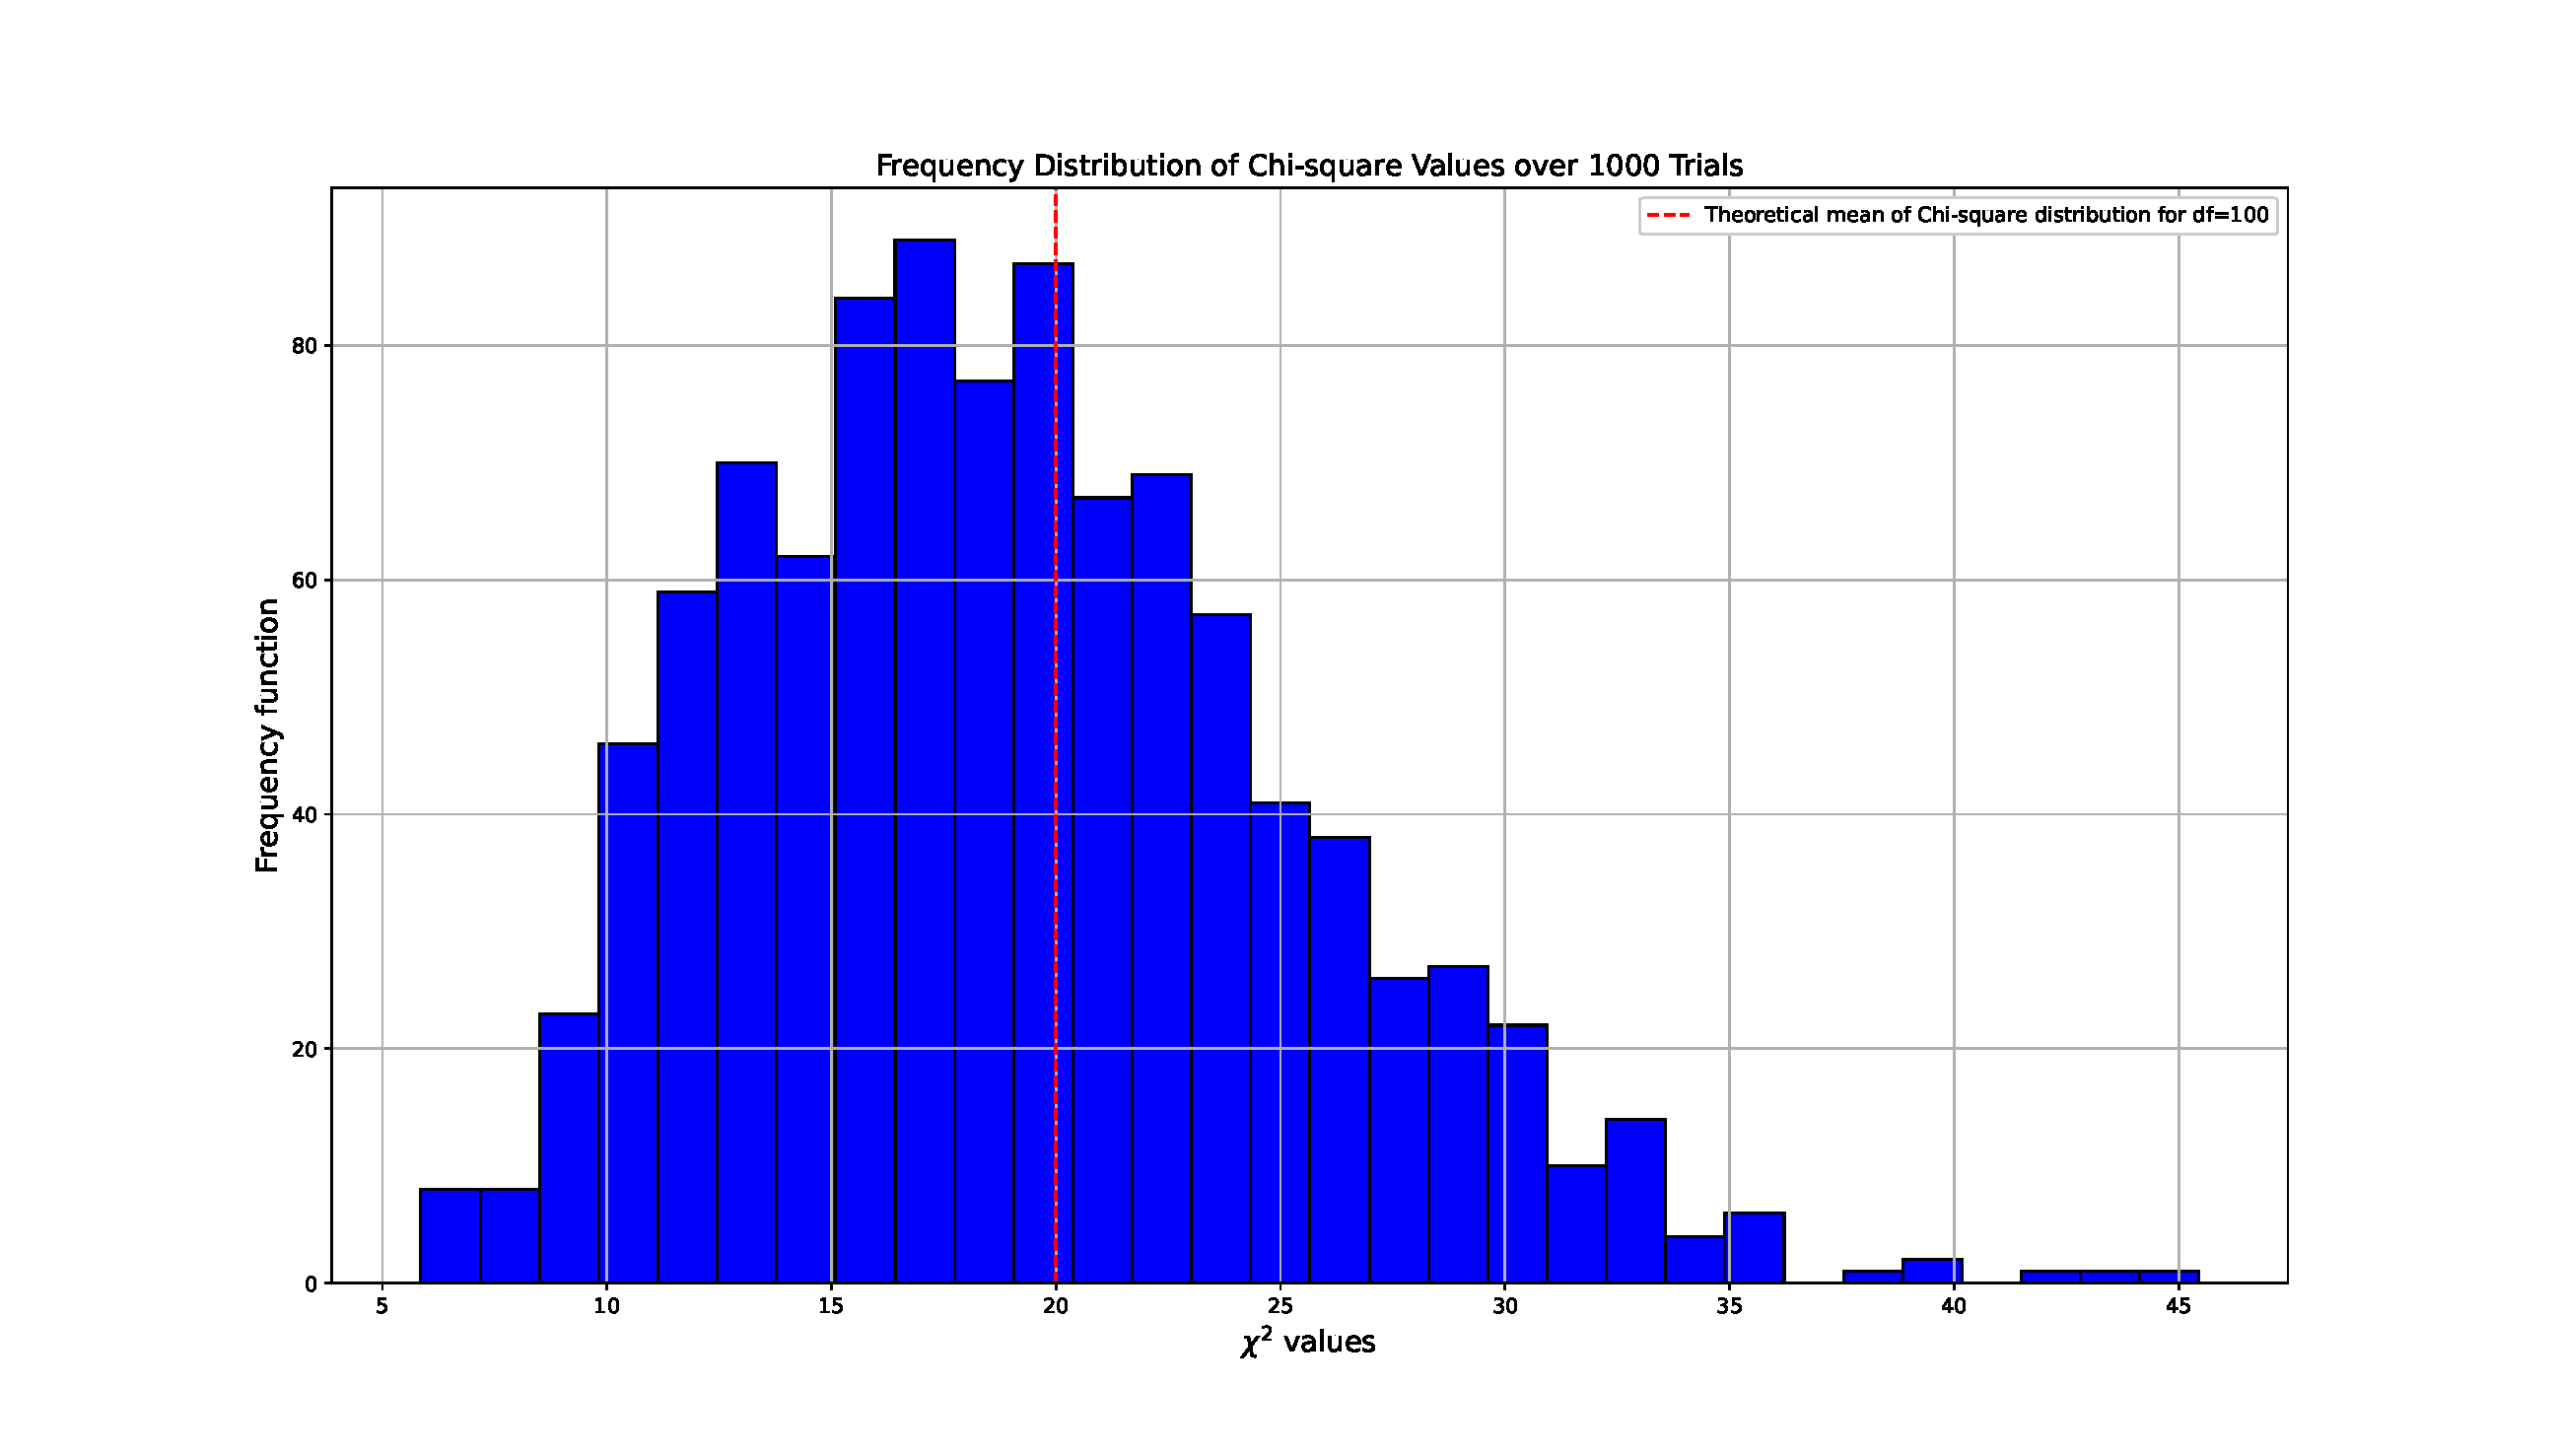
\includegraphics[height=0.32 \textheight]{1.6}
        \label{fig:1.6}
    \end{figure}

    不难发现,随着N的增大,模拟结果就越接近于理论情况,所以理想上的最佳结果是N越大越好。但实际情况中,往往在进行计算模拟时我们还需要考虑的计算所需的时间花费,模型所需的精度要求等等,所以最佳的选择要依靠实际问题来决定。

    \section{Problem2}\label{sec:2}
    \subsection{a}\label{subsec:2.1}
    利用 \texttt{Java} 代码,实现对 Ising model 的模拟,即 \(E, \, M\) 的计算,和翻转的实现,代码如下
    \begin{lstlisting}[language=Java, breaklines = true,label={lst:2.1.1}]
package property;

public class IsingModel1D {
    private double[] spins;
    private double J;
    private double h;
    private final int N;

    public IsingModel1D(double[] spins, double J, double h) {
        this.spins = spins.clone();
        this.J = J;
        this.h = h;
        N = spins.length;
    }

    public double energy() {
        double energy = 0;
        for (int i = 0; i < N; i++) {
            energy += -J * spins[i] * (spins[(i + 1 + N) % N] + spins[(i - 1 + N) % N]) / 2;
        }
        energy += -h * magnetisation();
        return energy;
    }

    public double magnetisation() {
        double mag = 0;
        for (int i = 0; i < spins.length; i++) {
            mag += spins[i];
        }
        return mag;
    }
    public double changeEnergy(int index) {
        var spinsNew = spins.clone();
        spinsNew[index] *= -1;
        var other = new IsingModel1D(spinsNew, J, h);
        return other.energy() - energy();
    }

    public void transform(int index) {
        spins[index] *= -1;
    }

}
    \end{lstlisting}

    在 Ising model 的基础上,我们改变了转移的机制,即恶魔模型中的随机选取一个自由度进行变换,\(\Delta E < E_d\) 时,采用该变换。

    利用 \texttt{Java} 代码实现如下
    \begin{lstlisting}[language=Java, breaklines = true,label={lst:2.1.2}]
package enterance;

import property.IsingModel1D;
import util.chat.Plot;

import static java.lang.StrictMath.*;
import static util.Vector.line;
import static util.Vector.value;

public class DemonAlgorithm {
    public static void main(String[] args) {
        int N = 100;
        double J = 1;
        double h = 0;
        double Ei = -20;
        double[] s = value(line(1, 1, N));
        var isingModel = new IsingModel(s, J, h);
        double Ed = isingModel.energy() + Ei;

        int steps = 1500;
        int warmSteps = 1000;
        var time = value(line(1, steps, steps));
        var energy = new double[steps];
        var mag = new double[steps];
        double avrEnergy = 0.0;
        double avrMag = 0.0;
        double avrMagSq = 0.0;

        for (int i = 0; i < steps; i++) {
            int index = (int) ((N - 1) * random());
            double delta = isingModel.changeEnergy(index);
            if (Ed <= delta) {
                isingModel.transform(index);
                Ed = isingModel.energy() + Ei;
            }
            energy[i] = isingModel.energy();
            mag[i] = isingModel.magnetisation();

            if (i > warmSteps) {
                avrEnergy += energy[i];
                avrMag += mag[i];
                avrMagSq += mag[i] * mag[i];
            }
        }

        avrEnergy /= (steps - warmSteps);
        avrMag /= (steps - warmSteps);
        avrMagSq /= (steps - warmSteps);

        System.out.println("Average energy: " + avrEnergy);
        System.out.println("Average Magnetisation: " + avrMag);
        System.out.println("Average Magnetisation Square: " + avrMagSq);

        var plot = new Plot(time, energy, mag);
        plot.setXLabel("Monte Calo steps");
        plot.setKeys("energy", "magnetisation");
        plot.draw();
    }
}
    \end{lstlisting}

    运行结果如下
    \begin{figure}[h]
        \centering
        \includegraphics[height=0.42 \textheight]{fig2_1_1}
        \caption{Ising model}\label{fig:2.1.1}
    \end{figure}
    \begin{figure}[h]
        \centering
        \includegraphics[height=0.12 \textheight]{fig2_1_2}
        \caption{平均值计算}\label{fig:2.1.2}
    \end{figure}

    \newpage
    \subsection{b}\label{subsec:2.2}
    利用题目提供的公式计算,利用 \texttt{Java} 代码实现如下
    \begin{lstlisting}[language=Java, breaklines = true,label={lst:2.2}]
package enterance;

import property.IsingModel1D;
import util.chat.Plot;

import static java.lang.StrictMath.*;
import static util.Vector.line;
import static util.Vector.value;

public class DemonAlgorithm {
    public static void main(String[] args) {
        int N = 100;
        double J = 1;
        double h = 0;
        double Ei = -20;
        double[] s = value(line(1, 1, N));
        var isingModel = new IsingModel(s, J, h);
        double Ed = isingModel.energy() + Ei;

        double kB = 1.380649 * pow(10, -23);
        double T = 4 * J / log(1 + 4 * J / Ed) / kB;
        System.out.println("T = " + T);
        System.out.println("M = " + (abs(Ed) / J));
    }
}
    \end{lstlisting}

    运行结果如下
    \begin{figure}[h]
        \centering
        \includegraphics[height=0.08 \textheight]{fig2_2}
        \caption{M 计算}\label{fig:2.2}
    \end{figure}

    \subsection{c}\label{subsec:2.3}
    利用题目所给公式计算,并与理论值进行比较,利用 \texttt{Java} 代码实现如下
    \begin{lstlisting}[language=Java, breaklines = true,label={lst:2.4}]
package enterance;

import property.IsingModel1D;
import util.chat.Plot;

import static java.lang.StrictMath.*;
import static util.Vector.line;
import static util.Vector.value;

public class DemonAlgorithm {
    public static void main(String[] args) {
        int N = 100;
        double J = 1;
        double h = 0;
        double[] Ei = {-40, -60, -80};
        double[] s = value(line(1, 1, N));
        var isingModel = new IsingModel1D(s, J, h);
        double E0 = isingModel.energy();
        var kT = new double[Ei.length];
        var MSq = new double[Ei.length];

        for (int i = 0; i < Ei.length; i++) {
            double Ed = E0 + Ei[i];
            kT[i] = 4 * J / log(1 + 4 * J / Ed);
            MSq[i] = abs(Ed) * abs(Ed) / J / J;
            System.out.println("kT = " + kT[i]);
            System.out.println("E = " + (E0 - Ed));
            System.out.println("exact E/N = " + (- tanh(J / kT[i])));
        }

        var plot = new Plot(kT, MSq);
        plot.setXLabel("kT");
        plot.setYLabel("MSq");
        plot.draw();
    }
}
    \end{lstlisting}

    运行结果如下
    \begin{figure}[h]
        \centering
        \includegraphics[height=0.42 \textheight]{fig2_4}
        \caption{M square 计算}\label{fig:2.4}
    \end{figure}
    \subsection{d}\label{subsec:2.4}

    \newpage
    \section{Problem3}\label{sec:3}
    \subsection{a}\label{subsec:3.1}
    对于此题,我们先利用随机数生成器随机的生成了一组二维自旋格子的构型,可视化如下:
    \begin{figure}[h]
        \centering
        \includegraphics[height=0.24 \textheight]{3.1.1}
        \label{fig:3.1.1}
    \end{figure}

    可以清晰地看到此时是具有无序性的。而后利用MCMC算法使系统达到平衡,并得到此时系统的能量,磁化强度,以及自旋模式的可视化图。

    具体结果如下:
    \begin{figure}[h]
        \centering
        \includegraphics[height=0.24 \textheight]{3.1.2}
        \label{fig:3.1.2}
    \end{figure}
    \begin{figure}[h]
        \centering
        \includegraphics[height=0.32 \textheight]{3.1.3}
        \label{fig:3.1.3}
    \end{figure}

    不难看出,此时在T=2的情形下,自旋模式出现一定的有序性,同时能量在50000步左右趋近与稳定,说明此时系统在经过50000步左右以后达到了一定的平衡状态。

    \subsection{b}\label{subsec:3.2}
    我们将上述在T=2的条件下运行的代码调整为在T=4的情形下运行即可,具体结果如下:
    \begin{figure}[h]
        \centering
        \includegraphics[height=0.24 \textheight]{3.2.1}
        \label{fig:3.2.1}
    \end{figure}
    \begin{figure}[h]
        \centering
        \includegraphics[height=0.32 \textheight]{3.2.2}
        \label{fig:3.2.2}
    \end{figure}

    从图中我们不难看出,在T=4的情形下,系统能量达到稳定情况时需要将近20000步,比(a)问中快了1倍有余。同时,系统的自旋模式出现有序性,基本所有的自旋格子都沿着同一个方向进行自旋。

    \subsection{c}\label{subsec:3.3}
    对于此题,我们固定了T=2,设置了三种有序的自旋模式:(1)自旋格子的自旋方向全部向上(2)自旋系统中75\%的自旋格子方向向上 (3)自选系统中45\%的自旋格子自旋方向向上。

    \newpage
    计算模拟结果如下:
    \subsubsection{1}\label{subsubsec:3.3.1}
    \begin{figure}[h]
        \centering
        \includegraphics[height=0.2 \textheight]{3.3.1}
        \label{fig:3.3.1}
    \end{figure}
    这一情况下,系统达到平衡状态所需要的步数远小于\(10^4\)步。

    \subsubsection{2}\label{subsubsec:3.3.2}
    \begin{figure}[h]
        \centering
        \includegraphics[height=0.2 \textheight]{3.3.2}
        \label{fig:3.3.2}
    \end{figure}
    这一情况下,系统达到平衡状态所需要的步数接近\(10^4\)步。

    \subsubsection{3}\label{subsubsec:3.3.3}
    \begin{figure}[h]
        \centering
        \includegraphics[height=0.2 \textheight]{3.3.3}
        \label{fig:3.3.3}
    \end{figure}

    这一情况下,系统达到平衡所需的步数在\(0.8\times10^5\)步左右。

    综上所述,初始自旋模式的有序性会显著影响系统达到平衡时所需要的步数,越是有序所需步数越少。

    \subsubsection{4}\label{subsubsec:3.3.4}
    为直观的看出相变温度在图上的体现,我们选择了两种初始自旋模式进行比较分析,一是75\%的自旋格子自旋方向向上,另一个是75\%的自旋格子自旋方向向下。从磁化强度的角度来看,在变化过程中,这两种模式的磁化强度会始终关于M=0有很好的对称性。结合题干条件画出图像如下:
    \begin{figure}[h]
        \centering
        \includegraphics[height=0.24 \textheight]{3.3.4.1}
        \label{fig:3.3.4.1}
    \end{figure}
    \begin{figure}[h]
        \centering
        \includegraphics[height=0.2 \textheight]{3.3.4.2}
        \label{fig:3.3.4.2}
    \end{figure}

    从图中不难看出,相变温度位于[2.0,2.5]区间内,与理论结果相接近。

    \subsection{e}\label{subsec:3.5}
    同上一问一样的思路,不过将L=30改为L=4,画出结果如下:
    \begin{figure}[h]
        \centering
        \includegraphics[height=0.24 \textheight]{3.5.1}
        \label{fig:3.5.1}
    \end{figure}
    \begin{figure}[h]
        \centering
        \includegraphics[height=0.24 \textheight]{3.5.2}
        \label{fig:3.5.2}
    \end{figure}

    从磁化强度的变化图中不难看出,其相变温度位于区间[1.5,2.0],但此时系统能量极其不稳定,所以可能因为此时自旋系统结构太小,与L→∞下的理论有所矛盾。

    \subsection{f}\label{subsec:3.6}
    在开放边界条件下,系统边缘的自旋格子只与系统内部相邻的自旋格子有相互作用,而与系统外没有,因此其可以看作是在周期性边界系统下增加了无序性得到的,因而可以预测其会导致系统达到稳定的时间变长。大致示意图如下:
    \begin{figure}[h]
        \centering
        \includegraphics[height=0.12 \textheight]{3.6}
        \label{fig:3.6}
    \end{figure}

    \subsection{g}\label{subsec:3.7}
    在这一题中,我们不再随机选择翻转的自旋格子,而是有序地选择自旋格子,大致示意图如下:
    \begin{figure}[h]
        \centering
        \includegraphics[height=0.32 \textheight]{3.7.1}
        \label{fig:3.7.1}
    \end{figure}
    \begin{figure}[h]
        \centering
        \includegraphics[height=0.32 \textheight]{3.7.2}
        \label{fig:3.7.2}
    \end{figure}
    从图中不难看出,相变温度仍然位于区间[2.0,2.5]之间,对于结果的影响并不大。这是因为所采取的MC步数足够大,导致随机选取在此时表现出的统计特性与顺序选取近乎于相同,所以两者的结果变化并不大。

    \subsection{h}\label{subsec:3.8}
    对于此处提到的两种做法,我们不难发现,如果在每个自旋翻转后都重新更新能量与磁化强度,因为每一步都是只有一个自旋格子进行翻转,所以需要更长的步数来使系统达到平衡,例如当L=30,共有\(2^{900}\)种构型,对其遍历所需的步数是极为庞大的。但与之相对的是,其结果是更容易预估的,更贴合物理实际的。而在每个MC步骤后再更新能量与磁化强度的话,因为每一步都可能有多个自旋翻转,能量与磁化强度的变化会更大,也就更容易达到系统的稳定状态。所以在这一方法下,达到系统平衡所需的步数会更少一点,但与之相对其每一步的结果会更难预估一点。

    \newpage
    \section{Problem4}\label{sec:4}
    \subsection{a}\label{subsec:4.1}
    类似前面的情况, 利用 \texttt{Python} 代码实现二维 Ising model,计算 \(M\) 相对与 \(T\) 的变化,代码如下
    \begin{lstlisting}[language=Python, breaklines = true,label={lst:4.1}]
import numpy as np
import matplotlib.pyplot as plt

def initialize_system(N):
    return np.random.choice([-1, 1], size=(N, N))

def calculate_energy(system, J):
    energy = 0
    for i in range(len(system)):
        for j in range(len(system)):
            energy += -J * system[i, j] * (
                system[(i+1) % len(system), j] +
                system[(i-1) % len(system), j] +
                system[i, (j+1) % len(system)] +
                system[i, (j-1) % len(system)]
            )
    return energy

def metropolis_step(system, J, k_B, T):
    N = len(system)
    for _ in range(N**2):
        i, j = np.random.randint(N, size=2)
        delta_E = 2 * J * system[i, j] * (
            system[(i+1) % N, j] +
            system[(i-1) % N, j] +
            system[i, (j+1) % N] +
            system[i, (j-1) % N]
        )
        if delta_E <= 0 or np.random.rand() < np.exp(-delta_E / (k_B * T)):
            system[i, j] *= -1

def simulate_2d_ising_model(N, J, k_B, T_range, equilibration_steps, measurement_steps):
    system = initialize_system(N)
    magnetizations = []

    for T in T_range:
        energy = calculate_energy(system, J)
        magnetization = np.sum(system) / (N**2)
        magnetizations.append(magnetization)

        # Equilibration steps
        for _ in range(equilibration_steps):
            metropolis_step(system, J, k_B, T)

        # Measurement steps
        for _ in range(measurement_steps):
            metropolis_step(system, J, k_B, T)
            magnetization = np.sum(system) / (N**2)
            magnetizations.append(magnetization)

    return magnetizations

# Constants
N = 20  # Size of the system (N x N)
J = 1.0  # Interaction strength
k_B = 1.0  # Boltzmann constant

# Simulation parameters
equilibration_steps = 1000
measurement_steps = 2000

# Temperature range
T_range = np.linspace(1.0, 4.0, 50)

# Perform simulation
magnetizations = simulate_2d_ising_model(N, J, k_B, T_range, equilibration_steps, measurement_steps)

# Plot magnetization versus temperature
plt.plot(T_range, magnetizations, marker='o')
plt.axvline(x=2.27, color='r', linestyle='--', label='Phase Transition')
plt.xlabel('Temperature (T)')
plt.ylabel('Magnetization (m)')
plt.title('Magnetization vs Temperature')
plt.legend()
plt.show()
    \end{lstlisting}

    运行结果如下
    \begin{figure}[h]
        \centering
        \includegraphics[height=0.42 \textheight]{fig_4_1}
        \caption{M - T}\label{fig:4.1}
    \end{figure}

    \subsection{b}\label{subsec:4.2}
    使用上述模型,研究 \(L\) 的影响,利用 \texttt{C++} 代码实现如下
    \begin{lstlisting}[language=C++, breaklines = true,label={lst:4.2}]
#include <iostream>
#include <fstream>
#include <vector>
#include <cmath>
#include <random>

// Function to initialize the 2D Ising lattice
void initializeLattice(std::vector<std::vector<int>>& lattice, int L) {
    std::random_device rd;
    std::mt19937 gen(rd());
    std::uniform_int_distribution<> dis(0, 1);

    for (int i = 0; i < L; ++i) {
        std::vector<int> row;
        for (int j = 0; j < L; ++j) {
            int spin = dis(gen) == 0 ? -1 : 1;
            row.push_back(spin);
        }
        lattice.push_back(row);
    }
}

// Function to calculate the magnetization of the 2D Ising model
double calculateMagnetization(std::vector<std::vector<int>>& lattice, int L) {
    double magnetization = 0.0;
    for (int i = 0; i < L; ++i) {
        for (int j = 0; j < L; ++j) {
            magnetization += lattice[i][j];
        }
    }
    return magnetization;
}

// Function to calculate the energy difference for a spin flip
double calculateDeltaE(std::vector<std::vector<int>>& lattice, int L, int i, int j) {
    int spin = lattice[i][j];
    int left = lattice[i][(j - 1 + L) % L];
    int right = lattice[i][(j + 1) % L];
    int up = lattice[(i - 1 + L) % L][j];
    int down = lattice[(i + 1) % L][j];
    return 2 * spin * (left + right + up + down);
}

// Function to perform a Monte Carlo step in the 2D Ising model
void monteCarloStep(std::vector<std::vector<int>>& lattice, int L, double J, double k_B, double T) {
    std::random_device rd;
    std::mt19937 gen(rd());
    std::uniform_real_distribution<> dis(0.0, 1.0);
    std::uniform_int_distribution<> disIndex(0, L - 1);

    for (int step = 0; step < L * L; ++step) {
        int i = disIndex(gen);
        int j = disIndex(gen);
        double delta_E = calculateDeltaE(lattice, L, i, j);

        if (delta_E <= 0 || dis(gen) < exp(-delta_E / (k_B * T))) {
            lattice[i][j] *= -1;
        }
    }
}

int main() {
    // Simulation parameters
    int L = 10;  // Size of the lattice (L x L)
    double J = 1.0;  // Interaction strength
    double k_B = 1.0;  // Boltzmann constant
    int numTemperatures = 100;  // Number of temperatures
    double minT = 1.0;  // Minimum temperature
    double maxT = 4.0;  // Maximum temperature
    int numEquilibrationSteps = 1000;  // Number of equilibration steps
    int numMeasurementSteps = 2000;  // Number of measurement steps

    // Temperature range
    std::vector<double> temperatures;
    for (int i = 0; i < numTemperatures; ++i) {
        double T = minT + i * (maxT - minT) / (numTemperatures - 1);
        temperatures.push_back(T);
    }

    // Output file
    std::ofstream outputFile("magnetization_data.txt");

    // Perform simulations for different temperatures and lattice sizes
    for (double T : temperatures) {
        for (int currentL = L; currentL <= 2 * L; currentL += L) {
            // Initialize the lattice
            std::vector<std::vector<int>> lattice;
            initializeLattice(lattice, currentL);

            double magnetization = calculateMagnetization(lattice, currentL);

            // Equilibration steps
            for (int step = 0; step < numEquilibrationSteps; ++step) {
                monteCarloStep(lattice, currentL, J, k_B, T);
            }

            // Measurement steps
            for (int step = 0; step < numMeasurementSteps; ++step) {
                monteCarloStep(lattice, currentL, J, k_B, T);
                magnetization = calculateMagnetization(lattice, currentL);
            }

            // Output lattice size, magnetization, and temperature to file
            outputFile << currentL << " " << magnetization << " " << T << std::endl;
        }
    }

    // Close the output file
    outputFile.close();

    std::cout << "Simulation completed. Results are saved in magnetization_data.txt." << std::endl;

    return 0;
}
    \end{lstlisting}

    运行结果如下
    \begin{figure}[h]
        \centering
        \includegraphics[height=0.42 \textheight]{fig_4_2}
        \caption{ln M^2 - ln L}\label{fig:4.2}
    \end{figure}

    \subsection{c}\label{subsec:4.3}
    磁化强度随着系统大小的增加,自旋和交互作用的数量也会增加。这可能会导致更复杂的行为和潜在的不同的相变特征。

    已知二维离子化模型的临界温度为Tc = 2.27。在温度低于Tc时,系统表现出自发磁化,而在Tc以上时,系统变得无序。改变温度范围可以揭示系统在不同温度条件下的行为。

    平衡和测量步骤的数量会影响模拟的收敛性。平衡步骤不足可能导致不准确的结果,而更多的测量步骤可以提供更准确的统计数据。

    \subsection{d}\label{subsec:4.4}
    使用上述模型,研究 \(L\) 的影响,利用 \texttt{Python} 代码实现如下
    \begin{lstlisting}[language=Python, breaklines = true,label={lst:4.4}]
import numpy as np
import matplotlib.pyplot as plt

# Set up the Ising model parameters
J = 1.0  # Interaction strength
k_B = 1.0  # Boltzmann constant
T_values = np.linspace(1.0, 3.0, 10)  # Temperature values

# Define the function to calculate M^2
def calculate_m_squared(lattice):
    return np.mean(lattice)**2

# Perform simulations for different L values
L_values = [4, 8, 16, 32]
m_squared_values = []

for L in L_values:
    m_squared_avg = []
    for T in T_values:
        lattice = np.random.choice([-1, 1], size=(L, L))
        m_squared = []
        for _ in range(1000):
            for _ in range(L**2):
                i, j = np.random.randint(0, L, size=2)
                delta_E = 2 * J * lattice[i, j] * (
                    lattice[(i-1)%L, j] + lattice[(i+1)%L, j] +
                    lattice[i, (j-1)%L] + lattice[i, (j+1)%L]
                )
                if delta_E <= 0 or np.random.rand() < np.exp(-delta_E / (k_B * T)):
                    lattice[i, j] *= -1
            m_squared.append(calculate_m_squared(lattice))
        m_squared_avg.append(np.mean(m_squared))
    m_squared_values.append(m_squared_avg)

# Transpose the m_squared_values array
m_squared_values = np.array(m_squared_values).T

# Plot ln(M^2) against ln(L)
for i, m_squared_avg in enumerate(m_squared_values):
    plt.scatter(np.log(L_values), np.log(m_squared_avg), marker='o', label="L="+str(L_values[i]))

plt.xlabel('ln(L)')
plt.ylabel('ln(M^2)')
plt.legend()
plt.show()
    \end{lstlisting}

    运行结果如下
    \begin{figure}[htbp]
        \centering
        \begin{subfigure}[b]{0.42\textwidth}
            \includegraphics[height=0.24 \textheight]{fig_4_4_1}
            \caption{L = 4}\label{fig:4.4.1}
        \end{subfigure}
        \hfill
        \begin{subfigure}[b]{0.42\textwidth}
            \includegraphics[height=0.24 \textheight]{fig_4_4_2}
            \caption{L = 8}\label{fig:4.4.2}
        \end{subfigure}
        \centering
        \begin{subfigure}[b]{0.42\textwidth}
            \includegraphics[height=0.20 \textheight]{fig_4_4_3}
            \caption{L = 16}\label{fig:4.4.3}
        \end{subfigure}
        \hfill
        \begin{subfigure}[b]{0.42\textwidth}
            \includegraphics[height=0.20 \textheight]{fig_4_4_4}
            \caption{L = 32}\label{fig:4.4.4}
        \end{subfigure}\label{fig:4.4}
    \end{figure}

    \subsection{e}\label{subsec:4.5}
    利用 Markov 链,制作出不同变化的情况,利用 \texttt{Python} 代码实现如下
    \begin{lstlisting}[language=Python, breaklines = true,label={lst:4.5}]
import numpy as np
import matplotlib.pyplot as plt
import matplotlib.animation as animation

# `设置模型参数`
L = 100  # `网格大小`
J = 1.0  # `相互作用强度`
k_B = 1.0  # `波尔兹曼常数`
T = 2.0  # `温度`

# `初始化二维伊辛模型`
lattice = np.random.choice([-1, 1], size=(L, L))

# `定义绘制函数`
def plot_lattice(i):
    plt.clf()
    plt.imshow(lattice, cmap='Greens' if lattice[0][0] == -1 else 'binary')
    plt.axis('off')

# `定义马尔科夫过程函数`
def monte_carlo_step():
    global lattice
    for _ in range(L * L):
        i, j = np.random.randint(0, L, size=2)
        delta_E = 2 * J * lattice[i, j] * (
            lattice[(i-1)%L, j] + lattice[(i+1)%L, j] +
            lattice[i, (j-1)%L] + lattice[i, (j+1)%L]
        )
        if delta_E <= 0 or np.random.rand() < np.exp(-delta_E / (k_B * T)):
            lattice[i, j] *= -1

# `创建动画帧`
fig = plt.figure()
frames = []
for i in range(1000):
    monte_carlo_step()
    if i % 100 == 0:
        frame = plt.imshow(lattice, cmap='Greens' if lattice[0][0] == -1 else 'binary')
        frames.append([frame])

# `创建动画`
ani = animation.ArtistAnimation(fig, frames, interval=100, blit=True)
ani.save('ising_animation.gif', writer='pillow')

plt.show()
    \end{lstlisting}

    从中截取几个图像如下
    \begin{figure}[htbp]
        \centering
        \begin{subfigure}[b]{0.42\textwidth}
            \includegraphics[height=0.24 \textheight]{fig_4_5_1}
            \label{fig:4.5.1}
        \end{subfigure}
        \hfill
        \begin{subfigure}[b]{0.42\textwidth}
            \includegraphics[height=0.24 \textheight]{fig_4_5_2}
            \label{fig:4.5.2}
        \end{subfigure}
        \centering
        \begin{subfigure}[b]{0.42\textwidth}
            \includegraphics[height=0.24 \textheight]{fig_4_5_3}
            \label{fig:4.5.3}
        \end{subfigure}
        \hfill
        \begin{subfigure}[b]{0.42\textwidth}
            \includegraphics[height=0.24 \textheight]{fig_4_5_4}
            \label{fig:4.5.4}
        \end{subfigure}
        \hfill
        \begin{subfigure}[b]{0.42\textwidth}
            \includegraphics[height=0.24 \textheight]{fig_4_5_5}
            \label{fig:4.5.5}
        \end{subfigure}
        \centering
        \begin{subfigure}[b]{0.42\textwidth}
            \includegraphics[height=0.24 \textheight]{fig_4_5_6}
            \label{fig:4.5.6}
        \end{subfigure}
        \caption{不同的模拟结果}\label{fig:4.5}
    \end{figure}

    \newpage
    \section{Problem5}\label{sec:5}
    类似一维 Ising model,实现三维 Ising Model。\texttt{Java} 代码如下
    \begin{lstlisting}[language=Java, breaklines = true,label={lst:5.1}]
package property;

import static java.lang.StrictMath.exp;
import static java.lang.StrictMath.random;

public class IsingModel3D {
    private double[][][] spins;
    private double J;
    private double h;
    private final int Nx;
    private final int Ny;
    private final int Nz;

    public IsingModel3D(double[][][] spins, double J, double h) {
        this.spins = spins.clone();
        this.J = J;
        this.h = h;
        Nx = spins.length;
        Ny = spins[0].length;
        Nz = spins[0][0].length;
    }

    public double energy() {
        double energy = 0;
        for (int i = 0; i < Nx; i++) {
            for (int j = 0; j < Ny; j++) {
                for (int k = 0; k < Nz; k++) {
                    energy += -J * spins[i][j][k] * (spins[(i + 1 + Nx) % Nx][j][k] + spins[(i - 1 + Nx) % Nx][j][k]
                + spins[(i + 1 + Nx) % Nx][(j + 1 + Ny) % Ny][k] + spins[(i - 1 + Nx) % Nx][(j - 1 + Ny) % Ny][k]
                + spins[(i + 1 + Nx) % Nx][j][(k + 1 + Nz) % Nz] + spins[(i - 1 + Nx) % Nx][j][(k - 1 + Nz) % Nz]
                + spins[(i + 1 + Nx) % Nx][(j + 1 + Ny) % Ny][(k + 1 + Nz) % Nz] + spins[(i - 1 + Nx) % Nx][(j - 1 + Ny) % Ny][(k - 1 + Nz) % Nz] ) / 2;
                }
            }
        }
        energy += -h * magnetisation();
        return energy;
    }

    public double magnetisation() {
        double mag = 0;
        for (int i = 0; i < Nx; i++) {
            for (int j = 0; j < Ny; j++) {
                for (int k = 0; k < Nz; k++) {
                    mag += spins[i][j][k];
                }
            }
        }
        return mag;
    }
    public double changeEnergy(int ix, int iy, int iz) {
        var spinsNew = spins.clone();
        spinsNew[ix][iy][iz] *= -1;
        var other = new IsingModel3D(spinsNew, J, h);
        return other.energy() - energy();
    }

    public void transform(int ix, int iy, int iz) {
        spins[ix][iy][iz] *= -1;
    }

    public void next(double kT) {
        for (int i = 0; i < Nx; i++) {
            for (int j = 0; j < Ny; j++) {
                for (int k = 0; k < Nz; k++) {
                    double delta = changeEnergy(i, j, k);
                    if(delta < 0) {
                        transform(i, j, k);
                    } else {
                        if (exp(- delta / kT) > random()) {
                            transform(i, j, k);
                        }
                    }
                }
            }
        }
    }
}
    \end{lstlisting}

    通过 \texttt{Ising3D.java} 实现题目要求的不同 \(kT\) 下的 \(E, \, M\) 的变化,代码如下
    \begin{lstlisting}[language=Java, breaklines = true,label={lst:5.2}]
package enterance;

import property.IsingModel3D;
import util.chat.Plot;

import java.awt.*;

import static java.lang.StrictMath.sqrt;
import static util.Vector.line;
import static util.Vector.value;

public class Ising3D {
    public static void main(String[] args) {
        int steps = 1500;
        int warmSteps = 1000;
        int n = 10;
        var spins = new double[n][n][n];
        for (int i = 0; i < n; i++) {
            for (int j = 0; j < n; j++) {
                for (int k = 0; k < n; k++) {
                    spins[i][j][k] = 1.0;
                }
            }
        }

        var kT = value(line(1, 10, 10));
        var energy = new double[kT.length];
        var mag = new double[kT.length];
        var magSq = new double[kT.length];
        for (int i = 0; i < kT.length; i++) {
            var isingModel3D = new IsingModel3D(spins, 1, 0);
            for (int j = 0; j < steps; j++) {
                System.out.println("kT " + kT[i] + " step " + j);
                isingModel3D.next(kT[i]);
                if (j > warmSteps) {
                    energy[i] += isingModel3D.energy();
                    mag[i] += isingModel3D.magnetisation();
                    magSq[i] += mag[i] * mag[i];
                }
            }
            energy[i] = energy[i] / (steps - warmSteps);
            mag[i] = mag[i] / (steps - warmSteps);
            magSq[i] = magSq[i] / (steps - warmSteps) - mag[i] * mag[i];
        }

        var plot1 = new Plot(kT, energy);
        plot1.draw();

        var m = new double[kT.length + 1][2][];
        m[0] = new double[][]{kT, mag};
        for (int i = 1; i < kT.length + 1; i++) {
            m[i][0] = new double[2];
            m[i][1] = new double[2];
            m[i][0][0] = kT[i - 1];
            m[i][0][1] = kT[i - 1];
            m[i][1][0] = mag[i - 1] + sqrt(magSq[i - 1]);
            m[i][1][1] = mag[i - 1] - sqrt(magSq[i - 1]);
        }

        var colors = new Color[m.length];
        colors[0] = Color.RED;
        for (int i = 1; i < kT.length + 1; i++) {
            colors[i] = Color.BLACK;
        }

        var plot2 = new Plot(m);
        plot2.setColors(colors);
        plot2.draw();
    }
}
    \end{lstlisting}

    运行结果如下
    \begin{figure}[htbp]
        \centering
        \begin{subfigure}[b]{0.42\textwidth}
            \includegraphics[height=0.24 \textheight]{fig5_1}
            \caption{E - kT}\label{fig:5.1}
        \end{subfigure}
        \hfill
        \begin{subfigure}[b]{0.42\textwidth}
            \includegraphics[height=0.24 \textheight]{fig5_2}
            \caption{M - kT}\label{fig:5.2}
        \end{subfigure}
        \caption{3D Ising model}\label{fig:5}
    \end{figure}

    通过计算可以得知,如果处理 \(1000\) 的,会出现数据溢出,\(100~1000\) 步才能让一个位型收敛是现在的 \(10 \times 10 \times 10 \times 10\) 倍,超出了 \texttt{double} 的最大范围。如果使用 \texttt{BigDecimal} 进行计算会带来更低的效率和更大的内存占用,这是电脑无法支撑的。
\end{document}
